\documentclass[../TV&MS.tex]{subfiles}
\begin{document}
    
\section{Случайные величины}

\subsection{Случайные величины: определение}

\qquad Случайные события "--- это хорошо, но события типа <<на монетке выпал герб>> плохо формализуемы, 
а мы хотим формальности и математичности. Поэтому вместо всяких событий хочется работать с числами. 
Вот этим и займемся. При рассмотрении случайных событий мы ввели вероятностное пространство, 
которое выглядит так:
$$(\Omega, \Ev, \Pro),$$

где $\Omega$ "--- множество элементарных событий, $\Ev$ "--- $\sigma$-алгебра подмножеств 
множества элементарных событий, а $\Pro$ "--- вероятность. Мы же будем рассматривать теперь тройку
$$(\Real, \Bor, \Pro),$$

где $\Real$ "--- действительная прямая, $\Bor$ "--- борелевская $\sigma$-алгебра, а $\Pro$ "--- вероятность.


Теперь формально введем понятие случайной величины (может использоваться сокращение с.в.).

\begin{Def}
Пусть $(\Omega, \Ev, \Pro)$ "--- вероятностное пространство. Тогда \mdef{случайной величиной $\xi$} 
называется функция $\xi : \Omega \to \Real$, измеримая относительно $\Ev$ и $\Bor$. 
По-другому, $\xi$ "--- случайная величина, если
$$\forall B \in \Bor \quad \xi^{-1}(B) = \lbrace \omega : \xi(\omega) \in B \rbrace \in \Ev.$$
\end{Def}

\begin{Wtf}
Таким финтом ушами мы по сути сопоставили каждому событию какое-то <<хорошее>> множество на 
числовой прямой, и можем рассматривать не вероятности событий, а вероятности попадания в эти 
<<хорошие>> подмножества числовой прямой.
\end{Wtf}

\subsection{Функция распределения}

Введем еще несколько <<полезных>> определений.

\begin{Def}
С каждой случайной величиной свяжем два вероятностных пространства: первое --- 
$(\Omega, \Ev_\xi, \Pro)$ --- вероятностное пространство, \mdef{порожденное $\xi$}. 
Здесь $\Ev_\xi$ - наименьшая $\sigma$-алгебра, для которой выполняется свойство измеримости. 
Второе --- $(\Real, \Bor, \Pro_\xi)$, где $\Pro_\xi(B) = \Pro(\xi^{-1}(B)) \quad \forall B \in \Bor$ 
и называется \mdef{распределением вероятностей $\xi$}.
\end{Def}

Идем дальше в~сторону упрощения работы со случайностями. Вместо того чтобы рассматривать произвольные 
борелевские множества, мы будем рассматривать только множества вида $(-\infty, x)$. Действительно, 
интервал $(a, b)$ получается из~полупрямых так: $(a, b) = (-\infty, b) \setminus (-\infty, a]$.  
Таким образом, мы можем рассматривать случайные величины только на таких множествах. Здесь имеется в виду, 
что для удовлетворения определению случайной величины достаточно измеримости только на
полупрямых, что следует из следующих свойств полного прообраза: прообраз объединения есть объединение 
прообразов, прообраз пересечения есть пересечение прообразов, прообраз отрицания есть отрицание прообраза. 
Выше показано, что из полупрямых с помощью этих операций можно получить интервалы, а из интервалов и все 
$\Bor$.

Теперь несколько полезных утверждений. Пусть $\xi$ --- случайная величина. Тогда $-\xi$ также 
случайная величина, так как её прообраз от любой полупрямой является прообразом $\xi$ от 
симметричной полупрямой, то есть лежит в $\Ev$. Величина $\xi + c$ также будет случайной величиной, 
поскольку ее прообразом для любой полупрямой будет прообраз $\xi$ для полупрямой, сдвинутой на $c$, 
то есть будет лежать в $\Ev$.

\begin{St}
Пусть $\xi, \eta$ --- случайные величины. Тогда множество $\left\{\omega \colon
\xi(\omega) < \right.$ $\left. \eta(\omega)\right\}$ является событием.
\end{St}
\begin{Proof}
$\Set{\omega}{\xi(\omega) < И\eta(\omega)} = \bigcup\limits_{r \in \mathbb{Q}}
\Set{\omega}{\xi(\omega) < r, \eta(\omega) > r}$. 
Заметим, что $\Set{\omega}{\xi(\omega) < r}$ является событием. Аналогично для $\eta$. 
Выражение, написанное выше, является счетным объединением пересечений двух событий, то есть событием.
\end{Proof}

Похожими махинациями, а также с использованием этого утверждения, доказывается, что 
$\xi^2, \xi + \eta, \xi\eta$ являются случайными величинами.
Более того, если $\xi_1, \ldots, \xi_n$~---~случайные величины, а функция $\phi(x_1, \ldots, x_n)$ 
является непрерывной на множестве их значений, то $\phi(\xi_1, \ldots, \xi_n)$ будет случайной 
величиной. 

\begin{Def}
Рассмотрим вероятностное пространство $(\Omega, \Ev, \Pro)$ и определенную на нем 
случайную величину $\xi$. Тогда её \mdef{функцией распределения $F_\xi(x)$}
называется функция $F_\xi : \Real \to \Real$
$$F_\xi(x) = \Pro(\omega : \xi(\omega) < x) = \Pro(\xi < x)$$.
\end{Def}

Запись $\Pro(\xi < x)$ является в некотором смысле жаргонной, так как аргументов 
вероятности должно быть событие из $\Ev$. Но $\xi < x$ мы в дальнейшем будем 
отождествлять с объединением элементарных событий, образ которых меньше $x$. Из определения 
случайной величины получаем, что это объединение является событием,
поэтому применение к нему функции вероятности корректно.

Функция распределения (сокращение ф.р.) является очень полезной штукой, поскольку имеет 
достаточно простой вид и несет в себе всю информацию о распределении, то есть однозначно 
определяет $\Pro_\xi$.

Рассмотрим основные свойства функции распределения:
\begin{enumerate}
	\item $F_\xi(x) \in [0, 1]$
	\item $\lim\limits_{x \to -\infty} F_\xi(x) = 0$
	\item $\lim\limits_{x \to +\infty} F_\xi(x) = 1$
	\item $F_\xi(x)$ монотонно не убывает.
	\item $F_\xi(x)$ непрерывна слева.
\end{enumerate}

Вероятность попадания с.в. в полуинтервал $\Pro_\xi[a,b) = F_\xi(b) - F_\xi(a)$. При 
стремлении $b \to a$ получим $\Pro(\xi = a) = F_\xi(a+0) - F_\xi(a)$, то есть 
вероятность попадания в точку равна скачку функции распределения в этой точке.

\begin{Def}
Точка $x_0$ называется \mdef{точкой роста} $F_\xi(x)$, если $\forall \varepsilon > 0 \quad$
$\Pro(x_0 -~\varepsilon \le \xi < x_0 + \varepsilon) > 0$
\end{Def}

\begin{Ex}
Это очень полезный пример, который будет использоваться в матстате и который очень любят спрашивать. 
Пусть $\xi$ --- случайная величина. $\eta = F_\xi(\xi)$. Чему равна $F_\eta(x)$? По определению 
\begin{equation}\label{fXiOfXi}
F_\eta(x) = \Pro(\eta < x) = \Pro(F_\xi(\xi) < x)=\Pro(\xi < F_\xi^{-1}(x)) = F_\xi(F_\xi^{-1}(x))=x
\end{equation}
Вообще, тут было бы неплохо сказать, что $F_\xi$ непрерывна и строго монотонна, чтобы со спокойной 
совестью использовать обратную функцию. Таким образом $\eta$ имеет равномерное распределение.
\end{Ex}

\subsection{Виды распределений}

Распределения случайных величин можно разделить на $3$ типа: непрерывные, дискретные и сингулярные.

\begin{Def}
	Случайная величина $\xi$ называется \mdef{абсолютно непрерывной}, если существует интегрируемая 
	функция $p_\xi(x) \ge 0, \ x \in \Real$ такая, что функция распределения $\xi$ является почти всюду 
	(за исключением не более, чем счетного числа точек) дифференцируемой функцией и представима в виде
	$$F_\xi(x) = \int\limits_{-\infty}^x p_\xi(y)dy$$
	Отсюда следует, что функция распределения непрерывна на $\Real$. $p_\xi(x)$ называется 
	\mdef{плотностью распределения}, и почти всюду выполнено $p_\xi(x)=F_\xi'(x)$.
	Плотность, вообще говоря, определена не однозначно.
\end{Def}

\begin{Def}
	Случайная величина $\xi$ называется \mdef{дискретной}, если множество точек роста не более, 
	чем счетно, но распределение не является сингулярным, или, 
	другими словами $\exists B = \{x_1, x_2, \ldots\} \colon \Pro(\xi \in B) = 1$.
\end{Def}

\begin{Def}
	Случайная величина $\xi$  называется \mdef{сингулярной}, если $F_\xi$ непрерывна, и 
	$\exists B \in \Bor \colon \mu(B) = 0, \ \Pro(\xi \in B) = 1$, то есть множество значений 
	случайной величины имеет меру 0, но вероятность попасть в каждую точку этого множества так же нулевая.
\end{Def}

Пара слов о жизненном смысле определений: непрерывная случайная величина имеет областью значений 
континуальное множество, при этом вероятность попасть в отдельно взятую точку нулевая. Пример: 
равномерное распределение по отрезку. Плотность же отражает вероятность попасть в ту или иную область: 
интеграл по области равен этой вероятности. Дискретная случайная величина принимает конечное или счетное 
множество значений, вследствие этого имеет ступенчатую функцию распределения, например, бросок монетки 
имеет дискретное распределение. Сингулярное распределение --- это крокодил, который не встречается в жизни 
и будет рассмотрен отдельно.

\begin{St}
	Дискретная случайная величина имеет не более, чем счетное число скачков.
\end{St}
\begin{Proof}
Из свойств функции распределения следует, что дискретная величина имеет не больше 
двух скачков величины больше $\frac12$. Аналогично, скачков величины больше $\frac13$ 
не больше $3$. То есть скачков величины больше $\frac1n$ не более $n$. Для любого скачка 
можно указать $n \in \mathbb{N}$ такое, что величина, этого скачка больше $\frac1n$. 
Значит,каждому скачку можно поставить в соответствие $n$, множество которых счетно. 
При этом для каждого $n$ существует не более чем счетное число скачков, ему соответствующих 
(величины $>\frac1n$). А так как объединение не более, чем счетного числа не более, чем 
счетных множеств, не более, чем счетно, получаем требуемое. 
\end{Proof}

\begin{Ex}
Для полного счастья приведем пример сингулярной случайной величины. Пусть функция 
распределения~---~так называемая лестница Кантора (см. рисунок).
\parbox[b][3 cm][t]{20mm}{\includegraphics[height=30mm]{kantor}}
\hfill
\parbox[b][3 cm][t]{100mm}{
	Посчитаем меру множества, на котором функция константа, то есть точки этого множества не 
	будут точками роста: сначала это одна ступенька длины $1/3$, потом две длины $1/9$, и т.\,д.
}\\
	$$ \frac13 + \frac29 + \frac4{27} = \frac13 \sum\limits_{k=1}^\infty(\frac23)^{k-1} = 1.$$

	Тогда множество точек роста имеет меру $0$ в силу свойства аддитивности меры.
\end{Ex}

Вообще говоря, существуют менее изысканные примеры сингулярных распределений. Например, при 
стрельбе из лука в круглую мишень распределение будет сингулярным, если стрелок попадает только 
в точки одной прямой. В самом деле, двумерная мера прямой равна $0$, как и вероятность 
попасть в каждую отдельную точку. 

\begin{Th} [Лебега]
	Любую случайную величину можно представить в виде суммы дискретной, абсолютно непрерывной и 
	сингулярной случайной величины. То есть 
	$$ F(x) = \alpha_dF_d(x) + \alpha_cF_c(x) + \alpha_sF_s(x), 
	\quad \alpha_d + \alpha_c + \alpha_s = 1.$$
\end{Th}
\begin{Proof}
Не вошло в содержание и не вышло с публикацией. Ищите в других учебниках.
\end{Proof}


\subsection{Векторные случайные величины}

	Векторную случайную величину можно определить двумя способами:
\begin{enumerate}
	\item Сказать, что $\xi = (\xi_1, \ldots, \xi_n)$ является векторной 
	случайной величиной, если ее координаты являются случайными величинами.

	\item Дать определение аналогично определению одномерной случайной величины, 
	то есть рассмотреть $(\Real^n, \Bor_n)$, где $\Bor_n$ --- $n$-мерная борелевская
	$\sigma$-алгебра, то есть минимальная $\sigma$-алгебра, содержащая все 
	параллелепипеды (аналогично интервалам в одномерном случае). 
	Тогда $\xi$~---~случайная величина, если 
	$$\forall B \in \Bor_n \colon \xi^{-1}(B) \in \Ev.$$ 
\end{enumerate}

\begin{Def}
	\mdef{Функция распределения векторной случайной величины} 
	$$F_\xi(x_1, \ldots, x_n) = \Pro(\xi_1 < x_1, \ldots, \xi_n < x_n).$$
\end{Def}

	Свойства функции распределения:
\begin{enumerate}
	\item Пусть $x, y \in \Real^n$ такие, что $x_i < y_i \quad i = 1, \ldots, n$. 
	Тогда $F_\xi(x) \leqslant F_\xi(y)$.

	\item $0 \leqslant F_\xi(x) \leqslant 1$.
	
	\item $\lim\limits_{x_i \to -\infty} F_\xi(x) = 0$. То есть при стремлении одной 
	координаты к $-\infty$ функция распределения стремится к $0$, поскольку вероятность 
	для соответствующей координаты стремится к $0$.
	
	\item Если же какую-то из координат устремить к бесконечности, то она не будет 
	учитываться в вероятности, поэтому
	$$\lim\limits_{x_i \to +\infty} F_\xi(x) = F_{(\xi_1, \ldots, \xi_{i-1}, \xi_{i+1}, 
	\ldots, \xi_n)}(x_1, \ldots, x_{i-1}, x_{i+1}, \ldots, x_n).$$

	\item Непрерывна слева по каждому аргументу.
\end{enumerate}

\begin{Def}
	\mdef{Абсолютно непрерывная} случайная величина $\xi$ --- такая случайная величина, что
	$$\forall B \in \Bor_n \quad \Pro(\xi \in \Bor_n) = 
	\int\limits_B p_\xi(x_1, \ldots, x_n)dx_1\ldots dx_n.$$ 
\end{Def}

	$\xi_1, \ldots, \xi_n$ независимы в совокупности $\Leftrightarrow$ функцию распределения 
	векторной случайной величины $\xi = (\xi_1, \ldots, \xi_n)$ можно представить 
	произведением функций распределений координат, то есть 
	$$F_\xi(x) = F_{\xi_1}(x_1)\ldots F_{\xi_n}(x_n).$$

	В случае абсолютно непрерывной векторной случайной величины это эквивалентно 
	аналогичному выражению для плотностей:
	$$p_\xi(x) = p_{\xi_1}(x_1)\ldots p_{\xi_n}(x_n).$$
	

\subsection{Условное математическое ожидание}

\subsubsection{Конструктивные определения}

\begin{Why}
    Уберите от экрана детей, беременных женщин и людей со слабой нервной системой.
	Сейчас будем вводить условное математическое ожидание. Для начала надо понять, 
	а где тут вообще проблема и почему нельзя ввести условную плотность как отношение 
	плотностей и тупо брать по ней интеграл. Во-первых, что такое матожидание?
	Матожидание~---~это простое обычное число. А теперь рассмотрим две случайные 
	величины: $\xi$ и $\eta$ и условное матожидание $\Expec(\xi|\eta)$.
	Пусть для наглядности $\xi$ "--- число, выпавшее на игральной кости, а $\eta$
	"--- остаток от деления на $2$ выпавшего числа. Тогда матожидание выпавшего числа 
	будет равно $4$, если известно, что выпало четное число, и $3$ "--- в противном случае.
	То есть матожидание зависит от условия, которое является случайной величиной, 
	а значит и само матожидание является случайной величиной.
	Таким образом, условное математическое ожидание мы не можем тупо определить как интеграл 
	от условной плотности, так как интеграл "--- это число. Поэтому мы введем условное 
	матожидание (УМО) отдельно для дискретных и непрерывных случайных величин, и в каждый раз 
	будем вводить этого крокодила в $2$ этапа. Сначала введем $\Expec(\xi | \eta = y)$ "--- 
	матожидание относительно конкретной реализации случайной величины. Это будет какая-то 
	функция от $y$. Потом скажем, что если в эту функцию подставить случайную величину $\eta$, 
	то мы получим $\Expec(\xi | \eta)$ "--- УМО относительно случайной величины.
	А потом еще для расширения сознания введем УМО относительно сигма-алгебры и 
	введем все то же, но по-другому, аксиоматически, а не конструктивно.
\end{Why}

	Пусть $\xi$ принимает значения $\{x_i\}$, а $\eta$ "--- $\{y_i\}$, тогда

\begin{Def}
    $\Expec(\xi | \eta = y_j) := 
    \sum\limits_{i} x_i \Pro(\xi = x_i | \eta = y_j) =
    \sum\limits_{i} x_i \dfrac{\Pro(\xi = x_i, \eta = y_j)}{\Pro(\eta = y_j)} = 
    f(y),\quad \text{где} y = y_j.$
\end{Def} 

\begin{Def}
    $\Expec(\xi | \eta) = f(\eta)$, где $f$ "--- функция, полученная с помощью
    предыдущего определения.
\end{Def} 

	Так как УМО "--- случайная величина, то мы можем взять матожидание этой 
	случайной величины и посмотреть, а что будет.

\begin{multline}
    \forall B \in \Bor \quad\Expec\bigl[ \Expec(\xi | \eta) \Ind(\eta \in B) \bigr] =
    \sum\limits_{j\colon y_j \in B} f(y_j) \Pro \left( \eta = y_j \right) = \\
    = \sum\limits_{j\colon y_j \in B} \left[\sum\limits_{k} x_k \frac{\Pro \bigl(\xi = 
    x_k, \eta = y_j\bigr)}{\Pro(\eta = y_j)} \right] \Pro (\eta = y_j) = \\
    = \sum\limits_{j\colon y_j \in B} \sum\limits_{k} \Pro\bigl(\xi = x_k, \eta = 
    y_j\bigr) = \Expec\bigl[\xi \Ind (\eta \in B)\bigr].
\end{multline}

	И в частности, если в качестве $B$ выбрать $\Real$, то индикатор всегда будет
	равен $1$ и тогда $\Expec\bigl[ \Expec (\xi | \eta) \bigr] = \Expec \xi$.

	Теперь рассмотрим абсолютно непрерывные случайные величины
	$\xi, \eta \sim p_{\xi, \eta}(x, y)$.
	Попробуем подступиться так же, как и в дискретном случае, через условную вероятность.

\begin{equation}
    \Pro(\xi < x | \eta = y) = 
    \frac{\Pro(\xi < x, \eta = y)}{\Pro(\eta = y)} = \frac{0}{0}.
\end{equation}

	Проблемка. Попробуем тогда у условии сказать, что
	$\eta \in [y, y + \varepsilon)$, и устремить $\varepsilon$ к нулю.

\begin{multline}
    \Pro \bigl(\xi < x | y \leqslant \eta < y + \varepsilon\bigr) =
    \frac{\Pro \bigl(\xi < x | y \leqslant \eta < y + \varepsilon\bigr)}
    {\Pro \bigl(y \leqslant \eta < y + \varepsilon\bigr)} = \\
    = \frac{\int\limits_{-\infty}^{x}\!\int\limits_{y}^{y + \varepsilon}
    p_{\xi, \eta}(x, y)dydx}{\int\limits_{y}^{y + \varepsilon} p_{\eta}(y)dy)} =
    \left\{ \text{\parbox{3.2cm}{считаем, что можно применить т. о среднем}} \right\} =
    \frac{\cancel{\varepsilon} \int\limits_{-\infty}^{x} p_{\xi,\eta}(x,y')dx}
    {\cancel{\varepsilon} p_\eta(y'')} = \\
    = \int\limits_{-\infty}^{x} \frac{p_{\xi, \eta}(x, y')dx}
    {p_\eta(y'')} \xrightarrow[\varepsilon \rightarrow 0]{} 
    \int\limits_{-\infty}^{x} \frac{p_{\xi, \eta}(x, y)}{p_\eta(y)}dx.
\end{multline}

	Теперь можем вводить определение условной плотности:

\begin{Def}
    $p_{\xi | \eta = y}(x) = \dfrac{p_{\xi, \eta}(x,y)}{p_\eta(y)}$.
\end{Def} 

\begin{Wtf}
    Условная плотность "--- функция от $x$, но параметризованная $y$.
\end{Wtf}

\begin{Def}
    $\displaystyle \Expec(\xi | \eta = y) := \int xp_{\xi | \eta = y}(x)dx = f(y).$
\end{Def}

	Теперь, как и в дискретном случае, конструктивно введем определение
	УМО относительно случайной величины.

\begin{Def}
    $\Expec(\xi | \eta) := f(\eta).$
\end{Def}

	И снова посчитаем МО УМО:

\begin{multline}
    \forall B \in \Bor \quad \Expec\bigl[ \Expec(\xi | \eta) \Ind(\eta \in B) \bigr] =
    \Expec\bigl[ f(\eta)\Ind(\eta \in B) \bigr] = \int\limits_{B} f(y)p_\eta(y)dy = \\
    = \int\limits_{B}\!\int x \frac{p_{\xi, \eta}(x, y)}{p_\eta(y)}dx\ p_\eta(y)dy=
    \int\limits_{B}\!\int xp_{\xi, \eta}(x, y)dxdy = 
    \Expec\bigl[\xi \Ind(\eta \in B) \bigr].
\end{multline} 

\subsubsection{Аксиоматическое определение}

	Теперь потихоньку будем вводить УМО через всякие там приколы с мерой.
	Вспомним наше любимое вероятностное пространство $(\Omega, \Ev, \Pro)$
	и рассмотрим некоторую под"--~$\sigma$"--~алгебру $\mathcal{F} \subseteq \Ev$.

\begin{Def}
    Случайная величина $\eta$ называется \mdef{$\mathcal{F}$"--~измеримой}, если 
    $$\forall B \in \Bor \quad \eta^{-1}(B) = \bigl\{\omega\colon\eta(\omega) 
    \in B)\bigr\} \in \mathcal{F}.$$
\end{Def} 

\begin{Wtf}
    Поясним: рассмотрим игральную кость.
    Тогда $\Omega = \left\{ 1, \ldots, 6 \right\}$,\ $\Ev = \left\{ 2^{\Omega} \right\}$.
    Теперь положим $\mathcal{F} = \bigl\{ \emptyset, 
        \left\{ 1, 3, 5 \right\},
        \left\{ 2, 4, 6 \right\},
        \Omega \bigr\}$.
      
    Теперь рассмотрим случайную величину $\eta$, которая равна чётности выпавшего числа.
    По определению легко проверяется, что $\eta$ является $\mathcal{F}$"--~измеримой.
\end{Wtf} 

\begin{Def}
    \mdef{Условным математическим ожиданием} случайной величины $\xi$ 
    относительно $\sigma$"--~алгебры $\mathcal{F}$ называется случайная
    величина $\Expec(\xi | \mathcal{F})$, обладающая следующими свойствами:
    \begin{enumerate}
        \item $\Expec(\xi | \mathcal{F})\ \mathcal{F}$"--~измерима.
        \item $\forall A \in \mathcal{F} \quad 
            \Expec\bigl[ \Expec(\xi | \mathcal{F}) \Ind(A) \bigr] =
            \Expec \bigl[ \xi \Ind(A) \bigr]$
    \end{enumerate} 
\end{Def}

	Введем теперь определение порожденной $\sigma$"--~алгебры.

\begin{Def}
    $\displaystyle \sigma(\eta) := 
    \bigcup\limits_{\forall B \in \Bor} \bigl\{\omega \colon \eta(\omega) \in B\bigr\}.$
\end{Def} 

\begin{Wtf}
    Это объединение всех множеств, которые мы получили следующим образом:
    берем борелевское множество, смотрим, какие события туда <<попадают>>,
    если перегнать из событий в $\Real$.
\end{Wtf} 

	И теперь, когда мы определили порожденную $\sigma$"--~алгебру,
	можно вводить аксиоматические определения для УМО относительно случайных величин.

\begin{Def}
    $\Expec(\xi | \eta) := \Expec(\xi | \sigma(\eta)).$
\end{Def} 

	Вообще по понятиям, если вводится такого рода определения, то надо доказывать 
	корректность таких определений. То есть мы определили какой-то новый объект, 
	но еще не факт, что такие крокодилы водятся в природе. Мы тут этим заниматься не будем, 
	чтобы не опухнуть от функана. Ключевые слова, чтобы казаться умным: мера, 
	абсолютно непрерывная относительно другой меры, теорема Рад\'{о}на"--~Ник\'{о}дима, заряд.

\subsubsection{Свойства и красивые картинки}

	Для начала запишем несколько свойств УМО (доказывать их я, конечно, не буду):
\begin{enumerate}
    \item $\forall B \in \Bor \quad \Pro\left( \xi \in B|\mathcal{F}\right)=
        \Expec\bigl[ \Ind(\xi \in B) | \mathcal{F} \bigr]$.
    
    \item $\Expec\bigl( a\xi_1 + b\xi_2 | \mathcal{F} \bigr) \Alsur
        a\Expec(\xi_1|\mathcal{F}) + b\Expec(\xi_2|\mathcal{F})$.

    \item Если $\eta\ \mathcal{F}$"--~измерима, то
        $\Expec(\xi\eta | \mathcal{F}) \Alsur \eta\Expec(\xi | \mathcal{F})$.

    \item Если $\xi$ и $\eta$ независимы, то
        $\Expec(\xi | \eta) \Alsur \Expec(\xi)$.

    \item $\Expec \bigl[ \Expec(\xi | \mathcal{F}) \bigr] = \Expec\xi$.
\end{enumerate} 

	Теперь картинки. Мы придумаем какую-нибудь плотность $p_{\xi,\eta}(x, y)$, 
	а потом построим график плотности условного матожидания и попытаемся понять
	его жизненный смысл.

	Чтобы было легко и просто мы представим плотность в таком виде:
\begin{equation}\label{gathEq}
    p_{\xi,\eta}(x,y) = p_{\xi|\eta}(x) p_{\eta}(y).
\end{equation}

	Затем положим:

\begin{equation}
     p_{\xi|\eta}(x) = \Norm(\eta, 1) = \frac{1}{\sqrt{2\pi}}
     exp\left\{ -\frac{(x-\eta)^2}{2} \right\},
\end{equation}

\begin{equation}
    p_\eta(y) = exp(1) = e^{-y}\Ind(y \geqslant 0).
\end{equation} 

	Теперь по понятиям. Что значит математическое ожидание $\xi$ при условии $\eta$?
	Это МО, если считать, что $\eta$ уже свалилось к нам с неба и не меняется.
	В силу построения условной плотности $\Expec(\xi | \eta) = \eta$ просто из 
	свойства нормального распределения. И полученная случайная величина, утверждается, 
	что распределена экспоненциально. Попробуем увидеть это на графиках.

\begin{figure}
\centering
\begin{minipage}[b]{0.5\textwidth}
    \centering
    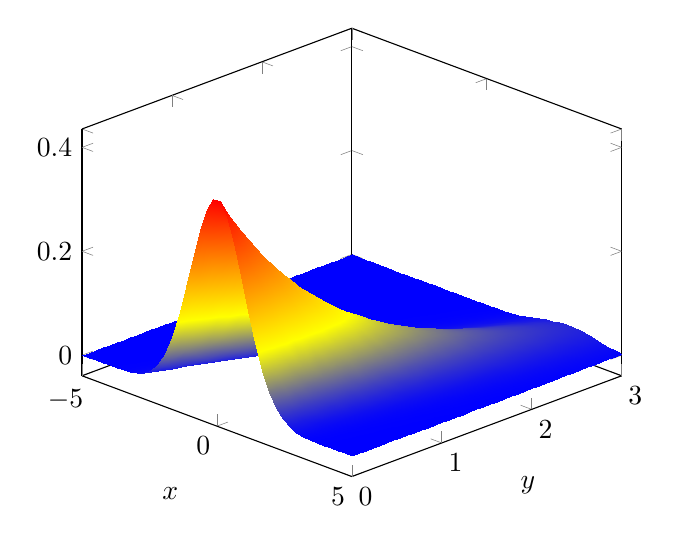
\begin{tikzpicture}
        \begin{axis}[view={45}{30},
            shader=interp,
            samples=40,
            domain y=0:3,
            xlabel=$x$,
            ylabel=$y$,
            ytick distance = 1,
            ]
            \addplot3[surf,
                domain=-5:5]
                {1/(sqrt(2*pi))*exp(-0.5*(x-y)^2 - y)};
        \end{axis} 
    \end{tikzpicture}
    \vfill
    \caption{Совместная плотность~\eqref{gathEq}.}
    \label{gathDensSide}
\end{minipage}%
\hfill
\begin{minipage}[b]{0.5\textwidth}
    \centering
    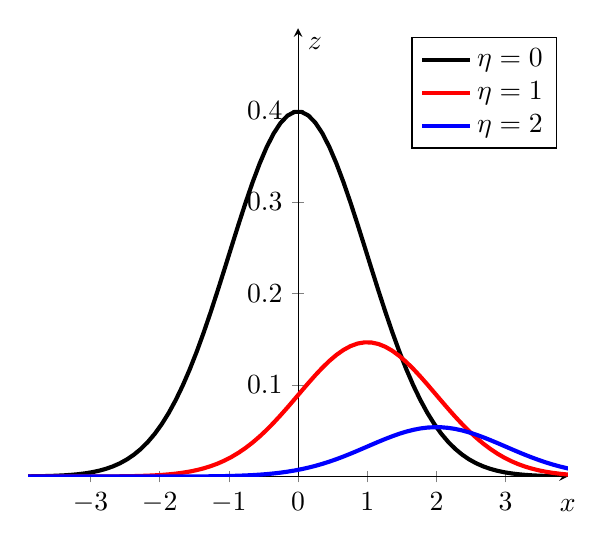
\begin{tikzpicture}
        \begin{axis}[
                ylabel=$z$,
                xlabel=$x$,
                xmin=-3.9,
                xmax=3.9,
                ymax = 0.49,
                xtick distance = 1,
                axis x line = bottom,
                axis y line = middle,
                samples=100,
                legend entries = {$\eta=0$, $\eta=1$, $\eta=2$},
                legend style = {fill=none},
                every axis x label/.style = {
                    at = {(ticklabel cs:1)}, anchor = south,
                },
                every axis plot/.style = {line width = 1.5pt,},
            ]
            \addplot[color=black]{1/(sqrt(2*pi))*exp(-0.5*x^2)};
            \addplot[color=red]{1/(sqrt(2*pi))*exp(-0.5*(x-1)^2 - 1)};
            \addplot[color=blue]{1/(sqrt(2*pi))*exp(-0.5*(x-2)^2 - 2)};
        \end{axis} 
    \end{tikzpicture}
    \vfill
    \caption{Сечения графика на рис.~\ref{gathDensSide} 
    		 при различных реализациях $\eta$.}
    \label{cutsGathDens}
\end{minipage}
\end{figure}

	Теперь если мы будем рассматривать сечения этого графика плоскостями
	$y=t, t \geqslant 0$, то будем получать каждый раз почти графики плотности
	нормального распределения с матожиданием $t$. Почему почти? Потому что 
	если проинтегрировать такой график, то получится число, меньшее $1$, 
	а именно равное вероятности (плотность имеет смысл вероятности) того, 
	что матожидание будет именно таким. Так что в данном конкретном случае 
	УМО можно увидеть на графике, рассматривая сечения при различных $y$.
	А вероятность попасть в то или иное УМО"---~это значение функции в максимуме
	при конкретном значении $y$ с поправкой на множитель $\frac{1}{\sqrt{2\pi}}$. 
	Если приглядеться, то можно увидеть, что вероятность попасть в матожидание
	убывает экспоненциально с ростом $y$, и так оно и должно быть в силу выбора
	$p_\eta(y)$. Конечно, не всегда все так красиво, это просто жалкая попытка 
	показать на картинке жизненный смысл всего этого безобразия.
\newpage
\end{document}
